\section{mo\-Gen\-Sol\-Continue$<$ EOT $>$ Class Template Reference}
\label{classmo_gen_sol_continue}\index{moGenSolContinue@{moGenSolContinue}}
One possible stop criterion for a solution-based heuristic.  


{\tt \#include $<$mo\-Gen\-Sol\-Continue.h$>$}

Inheritance diagram for mo\-Gen\-Sol\-Continue$<$ EOT $>$::\begin{figure}[H]
\begin{center}
\leavevmode
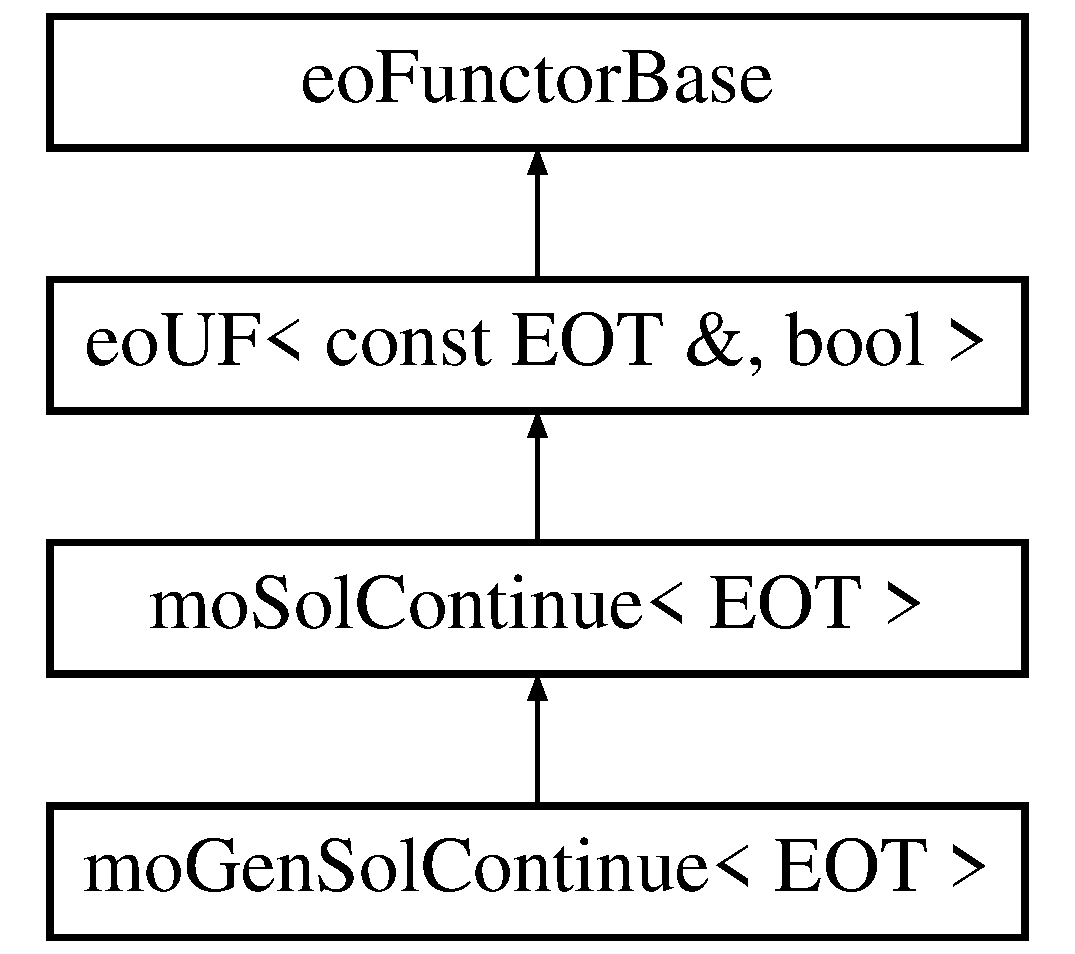
\includegraphics[height=4cm]{classmo_gen_sol_continue}
\end{center}
\end{figure}
\subsection*{Public Member Functions}
\begin{CompactItemize}
\item 
{\bf mo\-Gen\-Sol\-Continue} (unsigned int \_\-generation\-Maximum\-Number)
\begin{CompactList}\small\item\em Simple constructor. \item\end{CompactList}\item 
bool {\bf operator()} (const EOT \&\_\-solution)
\begin{CompactList}\small\item\em Function that activates the stop criterion. \item\end{CompactList}\item 
void {\bf init} ()
\begin{CompactList}\small\item\em Procedure which allows to initialise the generation counter. \item\end{CompactList}\end{CompactItemize}
\subsection*{Private Attributes}
\begin{CompactItemize}
\item 
unsigned int {\bf generation\-Maximum\-Number}\label{classmo_gen_sol_continue_r0}

\begin{CompactList}\small\item\em Iteration maximum number. \item\end{CompactList}\item 
unsigned int {\bf generation\-Number}\label{classmo_gen_sol_continue_r1}

\begin{CompactList}\small\item\em Iteration current number. \item\end{CompactList}\end{CompactItemize}


\subsection{Detailed Description}
\subsubsection*{template$<$class EOT$>$ class mo\-Gen\-Sol\-Continue$<$ EOT $>$}

One possible stop criterion for a solution-based heuristic. 

The stop criterion corresponds to a maximum number of iteration. 



Definition at line 46 of file mo\-Gen\-Sol\-Continue.h.

\subsection{Constructor \& Destructor Documentation}
\index{moGenSolContinue@{mo\-Gen\-Sol\-Continue}!moGenSolContinue@{moGenSolContinue}}
\index{moGenSolContinue@{moGenSolContinue}!moGenSolContinue@{mo\-Gen\-Sol\-Continue}}
\subsubsection{\setlength{\rightskip}{0pt plus 5cm}template$<$class EOT$>$ {\bf mo\-Gen\-Sol\-Continue}$<$ EOT $>$::{\bf mo\-Gen\-Sol\-Continue} (unsigned int {\em \_\-generation\-Maximum\-Number})\hspace{0.3cm}{\tt  [inline]}}\label{classmo_gen_sol_continue_a0}


Simple constructor. 

\begin{Desc}
\item[Parameters:]
\begin{description}
\item[{\em \_\-generation\-Maximum\-Number}]The maximum number of generations. \end{description}
\end{Desc}


Definition at line 54 of file mo\-Gen\-Sol\-Continue.h.

References mo\-Gen\-Sol\-Continue$<$ EOT $>$::generation\-Maximum\-Number, and mo\-Gen\-Sol\-Continue$<$ EOT $>$::generation\-Number.

\subsection{Member Function Documentation}
\index{moGenSolContinue@{mo\-Gen\-Sol\-Continue}!operator()@{operator()}}
\index{operator()@{operator()}!moGenSolContinue@{mo\-Gen\-Sol\-Continue}}
\subsubsection{\setlength{\rightskip}{0pt plus 5cm}template$<$class EOT$>$ bool {\bf mo\-Gen\-Sol\-Continue}$<$ EOT $>$::operator() (const EOT \& {\em \_\-solution})\hspace{0.3cm}{\tt  [inline, virtual]}}\label{classmo_gen_sol_continue_a1}


Function that activates the stop criterion. 

Increments the counter and returns TRUE if the current number of iteration is lower than the given maximum number of iterations.

\begin{Desc}
\item[Parameters:]
\begin{description}
\item[{\em \_\-solution}]The current solution. \end{description}
\end{Desc}
\begin{Desc}
\item[Returns:]true or false according to the current generation number. \end{Desc}


Implements {\bf eo\-UF$<$ const EOT \&, bool $>$}.

Definition at line 66 of file mo\-Gen\-Sol\-Continue.h.

References mo\-Gen\-Sol\-Continue$<$ EOT $>$::generation\-Number.\index{moGenSolContinue@{mo\-Gen\-Sol\-Continue}!init@{init}}
\index{init@{init}!moGenSolContinue@{mo\-Gen\-Sol\-Continue}}
\subsubsection{\setlength{\rightskip}{0pt plus 5cm}template$<$class EOT$>$ void {\bf mo\-Gen\-Sol\-Continue}$<$ EOT $>$::init ()\hspace{0.3cm}{\tt  [inline, virtual]}}\label{classmo_gen_sol_continue_a2}


Procedure which allows to initialise the generation counter. 

It can also be used to reset the iteration counter. 

Implements {\bf mo\-Sol\-Continue$<$ EOT $>$} {\rm (p.\,\pageref{classmo_sol_continue_a0})}.

Definition at line 78 of file mo\-Gen\-Sol\-Continue.h.

References mo\-Gen\-Sol\-Continue$<$ EOT $>$::generation\-Number.

The documentation for this class was generated from the following file:\begin{CompactItemize}
\item 
mo\-Gen\-Sol\-Continue.h\end{CompactItemize}
